\begin{figure}
    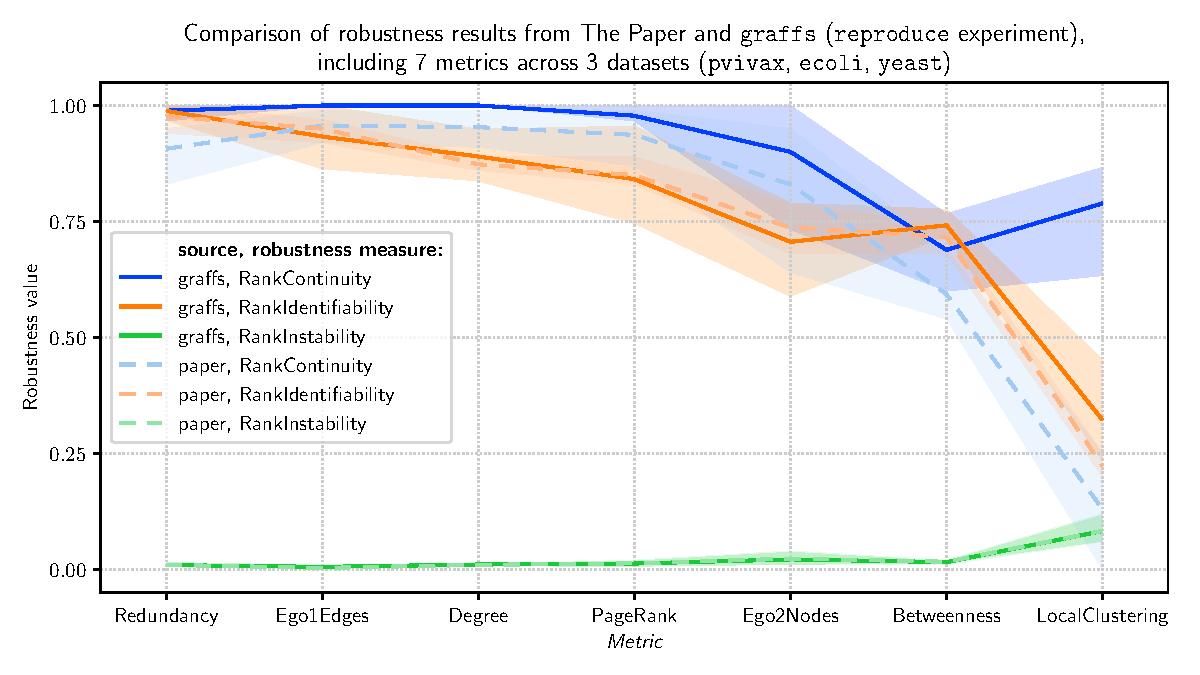
\includegraphics[width=\linewidth]{plot_reproduction.pdf}
    \vspace*{-0.6cm}
    \caption{Comparison of results from The Paper and \graffs.
    Each color corresponds to one robustness measure, with thin lines inside each band showing robustness of individual datasets, and the thick line showing the average robustness across the 3 datasets.
    Solid and dashed bands correspond to results obtained by \graffs and The Paper, respectively.}
    \label{fig:plot_reproduction}
    \footnotesize
    \begin{flushleft}
        Note that high values of RankContinuity and RankIdentifiability mean high \textsl{robustness}, whereas high values of RankInstability mean low \textsl{robustness}.
        Metrics are sorted from left to right by their decreasing combined robustness.
    \end{flushleft}
\end{figure}
